\pagebreak

Block name: GENARB\_f

Number of inputs: 0

Number of outputs: 1

Parameter list: Waveform Variable name, Sample rate

Block description: 
Arb Waveform (Arbitrary waveform generator) blocks, consisting of a current bank and a resistor, interface with the $\mu$P through memory mapped registers. The input is compiled as a vector on the SRAM. Run mode assembly code sends the input vector uploaded on SRAM to a memory mapped register at a given frequency.

\begin{figure}[H]  % jpg, png, or pdf
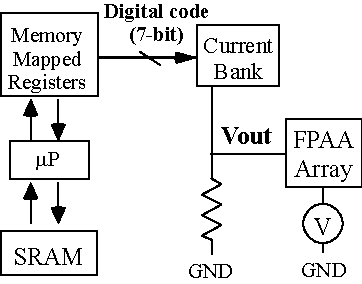
\includegraphics[width=300pt]{$FPAAHOME/rasp30/sci2blif/documentation/blocks_latex/figures/GENARB_f.pdf}
\end{figure}

